% Chapter Template

\chapter{Classification Algorithms} % Main chapter title

\label{Chapter4} % Change X to a consecutive number; for referencing this chapter elsewhere, use \ref{ChapterX}

\lhead{\emph{Classification Algorithms}} % Change X to a consecutive number; this is for the header on each page - perhaps a shortened title

%----------------------------------------------------------------------------------------
%	SECTION 1
%----------------------------------------------------------------------------------------

Machine learning algorithms are the fundamental of all classification program. 
These algorithms are divided in two big families: the supervised learning and the unsupervised learning.
In this project only supervised learning models are used.
This section presents briefly the classification algorithms used in this work. 
\section{Naïve Bayes classifier}
A Naïve Bayes classifier\cite{website:Naive_Bayes_classifier} is a simple probabilistic classifier based on applying Bayes' theorem (from Bayesian
statistics) with strong (naive) independence assumptions. 
In simple terms, a naive Bayes classifier assumes that the presence (or absence) of a particular feature of a class is unrelated to the presence (or absence) of any other feature.
Depending on the precise nature of the probability model, naive Bayes classifiers can be trained very efficiently in a supervised learning setting.

\subsection{The Naïve Bayes probabilistic model}
Abstractly, the probability model for a classifier is a conditional model.
$$ P(C|F_1, \cdots, F_n) $$

Over a dependent class variable $C$ with a small number of outcomes or $classes$, conditional on several feature
variables $F_1$ through $F_n$ . The problem is that if the number of features $n$ is large or when a feature can take on a
large number of values, then basing such a model on probability tables is infeasible. Therefore the
model is formulated to make it more tractable using Bayes' theorem:
$$ P(C|F_1, \cdots, F_n) = \frac{p(C)p(F_1, \cdots, F_n|C)}{p(F_1, \cdots, F_n)}$$  The equation could be formulated as follow in a literal way $$posterior = \frac{prior * likelihood}{evidence}$$


%----------------------------------------------------------------------------------------
%	SECTION 2
%----------------------------------------------------------------------------------------

\section{Support Vector Machine}
A Support Vector Machine (SVM) is a discriminative classifier formally defined by a separating hyperplane. In other words, given labeled training data (supervised learning), the algorithm outputs an optimal hyperplane which categorizes new examples.
The figure \ref{fig:hyperplane} shows an example for a linearly separable set of 2D-points which belong to one of two classes.
\begin{figure}[H]
  \centering
  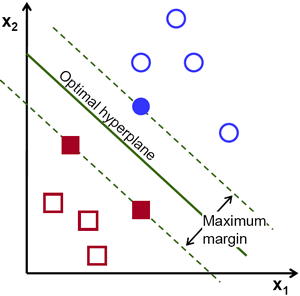
\includegraphics[width=60mm]{figures/optimal-hyperplane.png}
  \caption{Optimal hyperplane \label{fig:hyperplane}}
\end{figure}
The optimal hyperplane computedusing equation \ref{eq:hyperplane}:

\begin{equation}
\label{eq:hyperplane}
f(x) = \beta_{0} + \beta^{T} x
\end{equation}
Where $\beta$ is known as the weight vector and $\beta_{0}$ as the bias.

%----------------------------------------------------------------------------------------
%	SECTION 3
%----------------------------------------------------------------------------------------

\section{Maximum Entropy}
The maximum entropy classifier estimates probabilities
based on the principle of making as few
assumptions as possible, other than the constraints
imposed. Such constraints are derived from training
data, expressing some relationship between features
and outcome. The probability distribution
that satisfies the above property is the one with
the highest entropy. It is unique, agrees with the
maximum-likelihood distribution, and has the exponential
form :

\begin{equation}
\label{eq:maxent}
p(o|h) = \frac{1}{Z(h)}\prod_{j=1}^k\alpha_j^{f_j(h,o)}
\end{equation}

Where: 
\begin{itemize}
\item $o$ refers to the outcome
\item $h$ refers to the history or context.
\item $Z(h)$ is a normalization function.
\item $f_j(h,o)$ is a binary function.
\item $\alpha_j$ is estimated by a procedure called Generalized Iterative Scaling (GIS). This is an iterative method that improves the estimation of the parameters at each iteration.
\end{itemize}